\chapter{Úvod}
Tato práce se zabývá modely víceúrovňové autentizace. Jejím cílem je nalézt způsob pro přístup k jednomu zdroji z více univerzit za využití tamních přihlašovacích údajů.\\
Obsahuje základní informace o různých řešeních a dále se blíže zabývá modelem SSO v podobně standardu SAML a jeho konkrétní implementací Shibboleth.\\
Tato práce také obsahuje návody jak zprovoznit Shibboleth SP, napojit ho na různé poskytovatele identity což je ukázáno na Azure a SAMLtest, nastavení EDS pro využívání více IDP současně. A také využití Shibboleth SP s Apache2.\\


\section{Terminologie}
\subsection{Autentizace}
Proces ověření identity subjektu. Většinou následuje autorizace.\cite{Authorization}
\subsection{Autorizace}
Proces pro specifikování přístupových práv ke zdrojům.\cite{Autentizace}
 \subsection{Federované identity}
Způsob propojení identity uživatele napříč více nezávislými systémy. \cite{federatedIdentities}



\chapter{Modely víceúrovňové autentizace}
\section{SSO}
\label{sso}
SSO (Single Sign-On) je mechanizmus pro jednotné přihlášení. Umožňuje uživateli se přihlásit na jednom místě a následně využívat toto přihlášení pro přístup k více nezávislým aplikacím. \cite{SSO}

\section{Proxy autentizace}
Je mechanizmus udržení identity a práv uživatele skrze více úrovní. Znamená to že uživatel přistupuje celou dobu skrze aplikaci, na které se přihlásil, namísto přeposílání atributů třetí straně. Přihlašovací aplikace slouží tedy jako proxy server pro aplikaci třetí strany. \cite{ProxyA} \\ \\
Pro účely této práce není příliš vhodná jelikož většina implementací nemá možnost předávání atributů, nebo jiný způsob odlišení jednotlivých uživatelů od sebe.

\subsection{EZproxy}
Jedná se o proxy server používaný převážně knihovnami, pro udělování přístupu, k jejich zdrojům uživatelům v různých sítích. Autentizace probíhá převážně pomocí IP adresy.\\
EZproxy nemá žádný mechanizmus pro odlišování různých uživatelů. Používá se tedy například pro přístup ke zdrojům knihovny pro celé univerzity. \cite{EZproxy}\cite{wikiEZproxy}

\chapter{SSO}

Nejvhodnější model víceúrovňové autentizace pro tuto práci je SSO, jelikož se zabývá federovanými identitami a spousta univerzit již využívá nějakou implementaci SSO.
Dále je uvedeno několik jeho implementací pomocí různých standardů. 

\section{SAML}

SAML\cite{SAMLofficialSite}\cite{WhatIsSaml} (Security Assertion Markup Language) je otevřený standard umožňující výměnu autentizačních a autorizačních dat mezi více nezávislými subjekty. Využívá k tomu protokol XML. 

SAML definuje tři role. Uživatel, poskytovatel identity (zkráceně IDP) a poskytovatel služeb (zkráceně SP). 

IDP se stará o autentizaci uživatele a následné poskytnutí dat SP.

SP se stará o autorizaci uživatele ke svým zdrojům na základě informací poskytnutých od IDP.

\section{OIDC}

OIDC (OpenID Connect) je otevřený standard umožňující výměnu autentizačních a autorizačních dat mezi více nezávislými subjekty. Je postavený nad protokolem OAuth 2.0.\cite{OIDC}

\section{OAuth 2.0.}
Na rozdíl od OIDC OAuth 2.0. se stará pouze o autorizaci. Používá se většinou pro sdílení části dat uživatele s aplikací třetí strany, bez předávání jeho přihlašovacích údajů. \\
OIDC je potom jeho nadstavba určená přímo pro federované identity. \cite{OAUTHvSAMLvOIDC}

\section{SAML versus OIDC}

SAML je starší z těchto dvou protokolů a využívá k přenosu dat XML. OIDC je novější a využívá k přenosu dat JSON. 
SAML je momentálně rozšířenější i když OIDC nabírá na popularitě díky jednodušší implementaci a komunikaci přes JSON.\cite{SAMLxOIDC} \\
Princip přihlašování je až na různé názvosloví podobný (Service Provider (SP) = Relying Party (RP),  Identity Provider (IDP) = OpenID Provider (OP), atd ..).
Princip přihlašování je blíže popsán v sekci \ref{IDPlogin}.

\section{Shibboleth}

Shibboleth je implementace SAML standardu. Jeho hlavní součástí jsou dvě aplikace. Identity Provider (IDP), který slouží jako poskytovatel identity a stará se o autentizaci a Service Provider (SP), který slouží jako poskytovatel služeb a stará se o autorizaci po úspěšném přihlášení přes poskytovatele identity. \cite{shibbolethWiki}

\subsection{Poskytovatel identity}

Poskytovatel identity se stará o autentizaci uživatelů. Poskytovatel identity po autentizaci uživatele předá poskytovateli služeb informaci o úspěšné autentizaci společně s různými atributy (například: e-mal, uživatelské jméno, role atd...).

\subsection{Poskytovatel služeb}

Poskytovatel služeb se stará o autorizaci přístupu k různým službám, které poskytuje, na základě informací získaných od poskytovatele identity.

\subsection{Postup přihlášení za pomocí IDP}\label{IDPlogin}

Rozlišují se dvě možnosti přihlášení. Přihlášení vyvolané na straně IDP (obr. \ref{saml-flow-idp}) a přihlášení vyvolané na straně SP (obr. \ref{saml-flow-sp}).


Pokud bylo přihlášení vyvolané na straně SP, tak je uživatel přesměrován na IDP, kde bude vyzván k autentizaci.
Po úspěšné autentizaci IDP předá informaci o úspěšné autentizaci s různými uvolněnými atributy SP společně s přesměrováním uživatele na původní stránku.
Tyto informace SP využije k autorizaci různých svých částí uživateli.\cite{SAMLxOIDC}
\begin{figure}[bp]
	\centering
    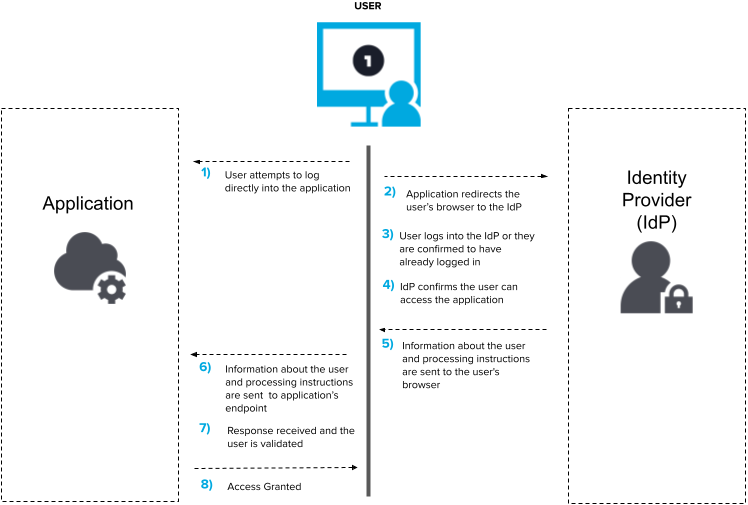
\includegraphics[width=1\textwidth]{obrazky-figures/saml-sp-cropped.png}
	\caption{Ukázka přihlášení vyvolané SP\cite{SAMLxOIDC}}
	\label{saml-flow-sp}
\end{figure}

Pokud bylo přihlášení vyvolané na straně IDP, tak je uživatel rovnou přesměrován na SP s informaci o úspěšné autentizaci společně s různými uvolněnými atributy.
Tyto informace SP využije k autorizaci různých svých částí.\cite{SAMLxOIDC}

\begin{figure}[bp]
	\centering
    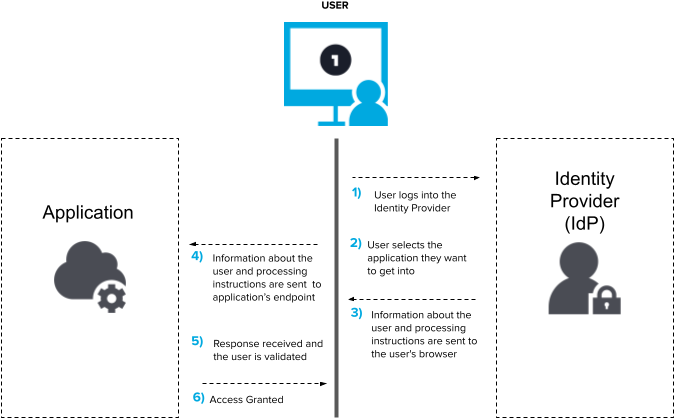
\includegraphics[width=1\textwidth]{obrazky-figures/saml-idp-cropped.png}
	\caption{Ukázka přihlášení vyvolané IDP\cite{SAMLxOIDC}}
	\label{saml-flow-idp}
\end{figure}
\chapter{Návod}
\label{návod}

Zde následuje návod jak nainstalovat a nastavit Shibboleth SP, tak aby ho bylo možné propojit s IDP. Jedná se převážně o aktualizaci tohoto návodu\cite{shibbolethSpInstallation}, v kombinaci s informacemi na oficiální wiki implementace Shibboleth\cite{shibbolethWikiSP}

\section{Instalace SP}

Nejdříve je třeba nainstalovat web server. Tento návod využívá Apache2
\begin{lstlisting}[language=Bash]
    sudo apt-get update
    sudo apt-get install apache2
\end{lstlisting}

Dále je třeba vygenerovat certifikáty pro Apache2. Pro jednoduchost se vygenerují self-signed certifikáty.
\begin{lstlisting}[language=Bash]
    sudo a2enmod ssl
    sudo a2ensite default-ssl.conf
    sudo mkdir /etc/apache2/ssl
    sudo openssl req -x509 -nodes -days 365 -newkey rsa:2048 \
    -keyout /etc/apache2/ssl/apache.key -out /etc/apache2/ssl/apache.crt
\end{lstlisting}

Shibboleth potřebuje vygenerovat certifikát ke komunikaci s IDP. Localhost je třeba nahradit ip adresou serveru na kterém SP poběží.
\begin{lstlisting}[language=Bash]
    sudo shib-keygen -h localhost
    openssl x509 -text -noout -in /etc/shibboleth/sp-cert.pem
\end{lstlisting}

Nastavení Shibboleth se nachází v /etc/shibboleth/shibboleth2.xml .

\begin{lstlisting}[language=Bash]
   sudo vim /etc/shibboleth/shibboleth2.xml
\end{lstlisting}

Zde je potřeba nastavit následující hodnoty. \\V <ApplicationDefaults> je potřeba nastavit EntityID. EntityID by mělo být jedinečné v rámci federace. Většinou se používá doména aplikace ke které se bude přistupovat přes Shibboleth s cestou /shibboleth. Například: http://vasedomena/shibboleth . Není to ale nutné pro fungování aplikace.

Pro povolení SSL je třeba nastavit v <Sessions>  handlerSSL na true a cookieProps na https.

Pod <SSO> se přidá EntityID IDP, který se bude používat.

Na konec souboru se přidá informace, kde se nachází metadata IDP.
\begin{lstlisting}[language=Bash]
 <MetadataProvider type="XML" validate="true"
                url="https://samltest.id/saml/idp"/>
\end{lstlisting}

pro jednoduchost se použije jeden klíč pro podpis i pro šifrování.

Toho se docílí změnou těchto řádků:
\begin{lstlisting}[language=Bash]
<CredentialResolver type="File" use="signing"
            key="sp-signing-key.pem" certificate="sp-cert.pem"/>
<CredentialResolver type="File" use="encryption"
            key="sp-encrypt-key.pem" certificate="sp-cert.pem"/>
\end{lstlisting}

na následující:
\begin{lstlisting}[language=Bash]
<CredentialResolver type="File"
            key="sp-key.pem" certificate="sp-cert.pem"/>
\end{lstlisting}

dále je třeba restartovat Shibboleth.
\begin{lstlisting}[language=Bash]
sudo service shibd restart
\end{lstlisting}

Pokud je vše nastaveno správně, tak na následující adrese bude text "A valid session was not found.".\\
\url{https://vasedomena/Shibboleth.sso/Session}

\section{Propojení s idp}

Zde je uvedeno pár návodů pro propojení SP s různými IDP.

\subsection{SAMLtest}
SAMLtest je testovací stránka pro debugování SAML aplikací. Většina IDP bude mít stejný postup propojení jako SAMLtest.



Na následující adresu je třeba nahrát metadata z SP 
\url{https://samltest.id/upload.php}. Ty se dají získat na následující cestě na doméně kde je hostován SP \url{https://vasedomena//Shibboleth.sso/Metadata}

dále je potřeba v nastavení Shibboleth SP (/etc/shibboleth/shibboleth2.xml) přidat cestu k metadatům IDP.
\begin{lstlisting}[language=Bash]
 <MetadataProvider type="XML"
                url="https://samltest.id/saml/idp"/>
\end{lstlisting}

Teď, když se zajde na stránku \url{https://samltest.id/start-sp-test/}, tak po vyplnění entityID se dá přihlásit do SP, přes SAMLtest IDP.

Po přihlášení by měly být vidět na následující adrese, informace o aktivní relaci \url{http://vasedomena/Shibboleth.sso/Session} 



\subsection{Azure}

Tato sekce je inspirována tímto návodem\cite{AzureTutorial}
\\
\\
Pro propojení s Azure IDP je potřeba udělat následující kroky
\begin{itemize}
    \item nejprve je potřeba vytvořit aplikaci, která bude sloužit jako IDP
    \begin{itemize}
    \item v Azure Portalu u Azure Services je třeba kliknout na Azure Active Directory
    \item vlevo ve sloupci pod manage otevřít Enterprise applications
    \item kliknout na New application
    \item kliknout na Create your own application
    \item tlačítkem Create potvrdit vytvoření aplikace
    \end{itemize}
    \item v aplikaci vlevo pod položkou Single sign-on se vybere SAML a dále je potřeba nastavit následující
    \item Basic SAML Configuration
    \begin{itemize}
        \item Identifier je třeba nastavit na entityID SP
        \item Reply URL je třeba nastavit na \url{https://vasedomena/Shibboleth.sso/SAML2/POST}
    \end{itemize}
    \item \mbox{Attributes \& Claims} \linebreak
    Protože Azure využívá pro NameID SAML identifier místo SAML atributu, tak je potřeba pro NameID nastavit Name identifier format na Unspecified.
    Dále stačí vybrat, jaký atribut se bude používat pro identifikaci uživatele.
    
    Po té je ještě potřeba v nastavení SP v souboru attribute-map.xml (/etc/shibboleth/attribute-map.xml) přidat následující řadky:
    
\begin{lstlisting}[language=XML]
   <Attribute name="urn:oasis:names:tc:SAML:1.1:nameid-format:unspecified"
   id="NameID">
        <AttributeDecoder xsi:type="NameIDAttributeDecoder" 
        formatter="$Name" defaultQualifiers="true"/>
   </Attribute>
\end{lstlisting}
které řeknou Shibboleth jak interpretovat NameID. NameID bude uloženo v proměnné NameID.

Jakékoli další atributy, které je potřeba předávat SP, se dají nastavit na této stránce podobným způsobem. Name format se nechá na Omitted, jinak zbytek nastavení je dle potřeb aplikace. Následně je potřeba do attribute-map.xml přidat informaci jak se mají jednotlivé atributy zpracovat.
   \begin{lstlisting}[language=XML]
     <Attribute name="Namespace/Name"
    nameFormat="urn:oasis:names:tc:SAML:2.0:attrname-format:unspecified"
    id="role1" />
    \end{lstlisting}
Namespace se nahradí za namespace atributu. Name se nahradí za název atributu a do id se nastaví název proměnné do které se má atribut namapovat. Pokud bylo potřeba měnit Name Format, tak je ho potřeba změnit i zde.\cite{AddAttribute}
    


    \item Dále je třeba nahrát pomocí tlačítka vlevo nahoře "Upload metadata file" metadata SP. Tato metadata jsou k nalezení na této cestě u vašeho SP \url{http://vasedomena/Shibboleth.sso/Metadata}

\end{itemize}

Po nastavení se dá aplikace otestovat tlačítkem Test. Aplikace by vás měla přesměrovat na doménu vaší aplikace a následně na následující adrese \url{https://vasedomena/Shibboleth.sso/Session} by měla být vidět aktivní relace a názvy atributů, které IDP předal SP.

\section{Používání v Apache}

Pro využití Shibboleth v Apache stačí uvést do .htaccess, co je vyžadováno za oprávnění od uživatele. Více informací o sytaxi je k nalezení v dokumentaci\cite{SPApache}\cite{SPhtaccess} \linebreak

příklad .htaccess pro přístup uživatele testuser@gmail.com:

 \begin{lstlisting}[language=xml]
    # nastavi typ prihlasovani na Shibboleth
    AuthType shibboleth
    # nastavi vyzadovani Shibboleth session
    ShibRequestSetting requireSession true
    # nasledujici blok nastavi ze je vyzadovana kombinace techto parametru
<RequireAll>
  # nastavi ze je vyzadovan shibboleth k pristupu
  require shibboleth 
  # nastavi pristup pro uzivatele s id testuser@gmail.com
  require shib-user testuser@gmail.com 
</RequireAll>
    \end{lstlisting}


\section{Discovery service}
Pro používání více než jednoho IDP je potřeba nastavit discovery service, kde si může uživatel vybrat jakého poskytovatele identity chce použít. Pro jednoduché řešení stačí statická webová stránka s přesměrováními na různé poskytovatele služeb, pro řešení obsahující více IDP je lepší využít discovery service od Shibboleth. Různé možnosti implementace jsou popsané v dokumentaci \cite{IdPDiscovery}.

\subsection{Embedded Discovery Service}
Je jednoduchá discovery service od Shibboleth napsaná v javascriptu. 

\subsection{Embedded Discovery Service - návod}
Tato sekce byla inspirována následujícím návodem \cite{EDS-tut}. \\ \\
instalace EDS:
\begin{lstlisting}[language=Bash]
sudo su -

cd /usr/local/src

wget https://shibboleth.net/downloads/embedded-discovery-service/\
latest/shibboleth-embedded-ds-1.2.2.tar.gz -O shibboleth-eds.tar.gz

tar xzf shibboleth-eds.tar.gz

cd shibboleth-embedded-ds-1.2.2

apt install make

make install
\end{lstlisting}

povolení webové stránky EDS

\begin{lstlisting}[language=Bash]
mv /etc/shibboleth-ds/shibboleth-ds.conf \
/etc/apache2/conf-available/shibboleth-ds.conf

a2enconf shibboleth-ds.conf

systemctl restart apache2.service
\end{lstlisting}

V Shibboleth SP nastavení (/etc/shibboleth/shibboleth2.xml), je třeba upravit následující:\\
 \begin{itemize}
    \item
SSO změnit následovně:

\begin{lstlisting}[language=Bash]
<SSO discoveryProtocol="SAMLDS" 
     discoveryURL="https://vasedomena/shibboleth-ds/index.html">
   SAML2 SAML1
</SSO>
\end{lstlisting}
\item
odkomentovat DiscoveryFeed handler a SessionInitiator handler

\begin{lstlisting}[language=xml]
<Handler type="DiscoveryFeed" Location="/DiscoFeed"/>
<Handler type="SessionInitiator" Location="/Login"/>
\end{lstlisting}
\end{itemize}
Následně je třeba restartovat Shibboleth SP a Apache2.

\begin{lstlisting}[language=Bash]
systemctl restart shibd.service
systemctl restart apache2.service
\end{lstlisting}

Dále je potřeba nastavit whitelist návratových adres v souboru idpselect\_config.js, který se nachází v nastavení EDS (/etc/shibboleth-ds/idpselect\_config.js)

v položce this.returnWhiteList je třeba změnit url aby odpovídala vašemu SP. 

\begin{lstlisting}[]
this.returnWhiteList = 
["^https:\/\/vasedomena\.com\/Shibboleth\.sso\/Login.*$",
 "^https:\/\/vasedomena\.com\/Shibboleth\.sso\/Login.*$"];
\end{lstlisting}

Teď když se zkusí zajít na na nějaký zdroj chráněný pomocí Shibboleth, tak dojde k přesměrování na stránku podobné té na obrázku \ref{EDS}.

\begin{figure}[bp]
	\centering
    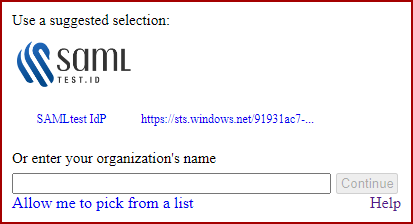
\includegraphics[width=0.6\textwidth]{obrazky-figures/disc.png}
	\caption{Ukázka EDS}
	\label{EDS}
\end{figure}

Zde si může uživatel jednoduše vybrat IDP, na jehož přihlašovací stránku chce být přesměrován.

\chapter{Config}
Popis důležitých částí nastavení, které jsou nutné k správnému fungování Shibboleth SP. Detailní informace jsou k nalezení na webu\cite{SPconfig}. 

\section{shibboleth2.xml}
Hlavní config soubor Shibboleth SP. Nachází se na cestě /etc/shibboleth/shibboleth2.xml .

\subsection{ApplicationDefaults}
\begin{lstlisting}[language=xml]
<ApplicationDefaults entityID="https://vasedomena/shibboleth"
        REMOTE_USER="NameID"
        cipherSuites="DEFAULT:!EXP:!LOW:!aNULL:!eNULL:!DES:!IDEA:
        !SEED:!RC4:!3DES:!kRSA:!SSLv2:!SSLv3:!TLSv1:!TLSv1.1">
\end{lstlisting}
\begin{itemize}
    \item entityID \linebreak
    Název SP. Musí být unikátní v rámci federace identit. Je zvykem využít doménu SP s cestou /shibboleth.  
    \item REMOTE\_USER \linebreak
    Zde patří názvy atributů od různých IDP, které slouží k identifikaci uživatele. 
    Tento atribut bude následně k dispozici z proměnné REMOTE\_USER.
\end{itemize}
\subsection{MetadataProvider}
Definuje kde se nachází metadata IDP. Pro většinu aplikací by mělo stačit jedno z následujících nastavení. Více informací lze nalézt na webových stránkách\cite{MetadataProvider}.
\linebreak \linebreak
Metadata se nahrávají z url.
\begin{lstlisting}[language=Bash]
 <MetadataProvider type="XML" validate="true"
                url="https://samltest.id/saml/idp"/>
\end{lstlisting}
Metadata se nahrávají ze souboru.
\begin{lstlisting}[language=Bash]
 <MetadataProvider type="XML" path="/path/to/the/metadata.xml"/>
\end{lstlisting}


\section{attribute-map.xml}
Obsahuje informace o mapování atributů přijatých od IDP na proměnné SP. Soubor obsahuje nějaké základní mapování, ale pro většinu aplikací bude nutné tento soubor upravit.

Následuje příklad přidání jednoduchého atributu, kde jméno atributu přijatého od IDP je FavoriteFruit a favFruit je jméno používané v proměnných SP\cite{AddAttribute}.
 \begin{lstlisting}[language=XML]
     <Attribute name="FavoriteFruit"
    nameFormat="urn:oasis:names:tc:SAML:2.0:attrname-format:basic"
    id="favFruit" />
    \end{lstlisting}
    
Toto nastavení by mělo být dostačující pro většinu aplikací. Více informací lze nalézt na webových stránkách\cite{AddAttribute}.

\chapter{Závěr}
V úvodu bylo prozkoumáno několik různých modelů pro víceúrovňovou autentizaci. Z těchto modelů bylo pro potřeby projektu zvoleno SSO, jelikož umožňovalo federovat identity uživatelů mezi více institucí s technologiemi, které již byli na těchto institucích většinou implementovány a také pro jednoduchou rozšiřitelnost o další instituce. 
\\
Z používaných technologií byl zvolen SAML, protože již existovala jeho implementace přímo pro potřeby univerzit a společně s OIDC patří k nejrozšířenějším SSO technologiím. \\
Touto implementací je Shibboleth, který je na řadě univerzit již implementován, nebo je implementován nějaký IDP, který je s ním kompatibilní (Azure, Google Suite, atd...).\\
Podařilo se nastavit Shibboleth SP pro základní přihlašování se dvěma poskytovateli identit (SAMLtest a Azure) a byly sepsány stručné návody pro základní zprovoznění SP, jeho napojení na 2 různé IDP, propojení s webovým serverem Apache2 a nastavení EDS pro využívání více IDP.

\label{zaver}






%===============================================================================
